\documentclass[11pt,letterpaper]{article}

\usepackage[margin=1in]{geometry}
\usepackage{lmodern}
\usepackage[T1]{fontenc}
\usepackage[utf8]{inputenc}
\usepackage{microtype}
\usepackage{amsmath,amssymb,amsthm}
\usepackage{mathtools}
\usepackage{xcolor}
\usepackage[most]{tcolorbox}
\usepackage{booktabs}
\usepackage{longtable}
\usepackage{array}
\usepackage{enumitem}
\usepackage{fancyhdr}
\usepackage{titlesec}
\usepackage{listings}
\usepackage{tikz}
\usetikzlibrary{shapes.geometric,arrows.meta,positioning,fit,backgrounds,calc}
\usepackage[hidelinks]{hyperref}

% Palette
\definecolor{KuklaInk}{HTML}{1B2A4A}
\definecolor{KuklaAccent}{HTML}{8C4F2B}
\definecolor{KuklaMath}{HTML}{FAF6EE}
\definecolor{KuklaSky}{HTML}{D9E4F5}
\definecolor{KuklaGreen}{HTML}{2E5E3A}
\definecolor{CodeBG}{HTML}{F4F2ED}

\titleformat{\section}{\Large\bfseries\color{KuklaInk}}{\thesection}{0.6em}{}
\titleformat{\subsection}{\large\bfseries\color{KuklaAccent}}{\thesubsection}{0.5em}{}
\titleformat{\subsubsection}{\normalsize\bfseries\color{KuklaInk}}{\thesubsubsection}{0.5em}{}

\pagestyle{fancy}
\fancyhf{}
\fancyhead[L]{\small\color{KuklaInk}\textbf{OSTI-x-CARDS} — System \& Methods}
\fancyhead[R]{\small\thepage}
\renewcommand{\headrulewidth}{0.4pt}
\renewcommand{\headrule}{\hbox to\headwidth{\color{KuklaInk}\leaders\hrule height \headrulewidth\hfill}}

\newtcolorbox{notebox}[1]{
  enhanced, breakable,
  colback=KuklaSky, colframe=KuklaInk,
  fonttitle=\bfseries\color{white}, coltitle=white,
  attach boxed title to top left={xshift=10pt,yshift=-8pt},
  boxed title style={colback=KuklaInk,sharp corners},
  title={#1}, arc=2mm, boxrule=0.8pt,
}

\newtcolorbox{rulebox}[1]{
  enhanced, breakable,
  colback=KuklaMath, colframe=KuklaAccent,
  fonttitle=\bfseries\color{KuklaAccent}, coltitle=KuklaAccent,
  title={#1}, arc=1mm, boxrule=0.5pt,
}

\lstdefinelanguage{yaml}{
  keywords={true,false,null},
  comment=[l]{\#},
  morestring=[b]",
}
\lstdefinestyle{sh}{
  basicstyle=\ttfamily\footnotesize, backgroundcolor=\color{CodeBG},
  breaklines=true, frame=single, rulecolor=\color{KuklaInk!30},
  framesep=4pt, xleftmargin=4pt, xrightmargin=4pt, aboveskip=6pt, belowskip=6pt,
  keywordstyle=\color{KuklaInk}\bfseries, commentstyle=\color{KuklaGreen}\itshape,
}
\lstset{style=sh}

\newcommand{\code}[1]{\texttt{\small #1}}

\title{\color{KuklaInk}\Huge\textbf{OSTI-x-CARDS}\\[6pt]
  \large\color{KuklaAccent}Turning 235{,}000 DOE Scientific Papers into\\
  Structured, Agent-Actionable Knowledge Cards\\[10pt]
  \normalsize\color{KuklaInk}\emph{Architecture, Workflows, Templates, Parsing, Fetching, and Serving}}
\author{Kukla \\ \small Hermes Agent / M1 Mac mini \\ \small \texttt{github.com/rick-stevens-ai/OSTI-x-CARDS}}
\date{\today}

\begin{document}
\maketitle
\thispagestyle{fancy}

\begin{abstract}
\noindent
\textbf{OSTI-x-CARDS} is an end-to-end knowledge-extraction system that converts the
U.S.\ Department of Energy's Office of Scientific and Technical Information (OSTI)
corpus --- roughly \textbf{234{,}705} scientific papers --- into \emph{x-Cards}:
structured, machine-readable records describing the research \emph{resources} each
paper introduces or uses (datasets, trained models, software agents, instruments,
user facilities, simulation codes, and computational workflows). Papers are fetched
from OSTI, parsed on GPU with Marker and Nougat, read by an LLM farm that emits
seven-modality cards, quality-scored against a four-component rubric, enriched by
zero-hallucination cross-card fact transfer, merged into consensus \emph{SuperCards}
per real-world resource, and rendered as review/tutorial articles. The result is
served through a FastAPI web interface and a Model Context Protocol (MCP) server for
direct agent access. As of this writing the system holds \textbf{311{,}188} x-Cards
across \textbf{134{,}956} distinct papers and \textbf{18{,}862} SuperCards
consolidating \textbf{155{,}110} member cards. This paper documents the complete
system: the data model, the batch pipeline stage by stage, the LLM infrastructure,
the card and review templates, the quality and enrichment methodology, the SuperCard
entity-resolution strategy, and the serving layer --- together with the engineering
principles (zero hallucination, restartability, replace-on-improvement, honest
tiering) that govern every stage.
\end{abstract}

\vspace{0.5em}
\tableofcontents
\clearpage

% ======================================================================
\section{Introduction and Motivation}
% ======================================================================

The DOE national-laboratory complex produces an enormous, continuously growing
literature. OSTI is its public clearinghouse: journal articles, conference papers,
and technical reports, each with a stable OSTI identifier and (often) a full-text
PDF. For a human researcher this corpus is navigable one paper at a time. For an
\emph{autonomous agent} --- the kind of system that now plans experiments, writes
analysis code, and reasons over scientific infrastructure --- a pile of PDFs is
nearly useless. What an agent needs is not prose but \emph{structured, grounded,
queryable facts about reusable research resources}: which dataset was released,
where it lives, under what license; which simulation code was used, at what version;
which instrument at which facility produced the measurements; which software agent
was built and what it can do.

OSTI-x-CARDS exists to manufacture exactly that layer. It reads the corpus and
distills, from each paper, the \emph{resources} it describes into a fixed schema of
seven modalities. Each distilled record is an \textbf{x-Card}. Cards are then
quality-graded, cross-linked, enriched, and merged so that a resource mentioned in
three thousand papers (say, the VASP simulation code, or the Advanced Photon Source)
becomes one authoritative \textbf{SuperCard} with an evidence-weighted consensus
record and a synthesized review article. Everything is served to both humans (a
browsable web site) and machines (an MCP server).

\begin{notebox}{What problem is being solved}
A corpus of unstructured PDFs is converted into a structured, agent-actionable
knowledge base of \emph{research resources}, with every fact traceable to a source
OSTI record and nothing fabricated. The deliverable is not a search engine over
papers; it is a \emph{resource catalogue} extracted from papers.
\end{notebox}

\subsection{What is in an x-Card}

Each x-Card captures one research resource from one paper, in one of seven
modalities. The modality determines the required fields and the review-article
section template.

\begin{center}
\small
\begin{tabular}{@{}l l l@{}}
\toprule
\textbf{Modality} & \textbf{Captures} & \textbf{Example resource} \\
\midrule
\code{data}       & Published datasets            & FLUXNET2015 eddy-covariance flux data \\
\code{model}      & Trained/parametric models     & A crystallography refinement model \\
\code{agent}      & Autonomous software agents    & Peregrine (ORNL additive-mfg.\ agent) \\
\code{instrument} & Physical measurement devices  & X-ray streak camera at APS Sector 7 \\
\code{facility}   & User facilities / infrastructure & Advanced Photon Source; NERSC \\
\code{simulation} & Simulation / modeling codes   & VASP; LAMMPS \\
\code{workflow}   & Computational pipelines       & Genomics variant-calling workflow \\
\bottomrule
\end{tabular}
\end{center}

\subsection{Current scale (live snapshot)}

The numbers below are read directly from the running service's
\code{/api/stats} and \code{/api/supercards/stats} endpoints.

\begin{center}
\small
\begin{tabular}{@{}l r@{}}
\toprule
\textbf{Quantity} & \textbf{Value} \\
\midrule
Corpus universe (Journal + Conference + Tech.\ Report) & 234{,}705 papers \\
x-Cards extracted (real, excl.\ sentinels)             & 311{,}188 \\
Distinct papers with $\geq 1$ card                     & 134{,}956 \\
SuperCards (consolidated resources)                    & 18{,}862 \\
SuperCard member cards                                 & 155{,}110 \\
Cards with official DOE subject classification         & 193{,}000+ \\
\bottomrule
\end{tabular}
\end{center}

\noindent Card counts by modality: instrument 82{,}777; facility 71{,}108;
simulation 66{,}039; workflow 50{,}855; model 20{,}036; data 18{,}276; agent 2{,}097.
The corpus spans publication years 2000--2026, with the bulk (${>}20$k cards/year)
concentrated in 2018--2025.

\begin{rulebox}{The four governing principles}
\textbf{(1) Zero hallucination.} Emails, URLs, and versions are recorded only if
observed in paper text, a sibling card, or a verified contact database --- never
pattern-constructed.
\textbf{(2) Review/tutorial, not sparse outlines.} Cards and SuperCards render as
synthesized explanatory articles grounded in the source papers with inline
\code{[OSTI:id]} citations.
\textbf{(3) Replace-on-improvement.} Enrichment never regresses a good card; QA
writes new columns and new versions, never destructively overwrites.
\textbf{(4) Restartable at every stage.} Farm jobs claim work atomically and resume;
a kill loses only in-flight items.
\end{rulebox}

\clearpage
% ======================================================================
\section{System Architecture}
% ======================================================================

OSTI-x-CARDS is a \emph{batch knowledge-extraction pipeline feeding a read-serving
layer}. Every stage is SQLite-backed, farm-parallel at the LLM-heavy steps, and
restartable. The design deliberately separates slow, expensive, offline enrichment
(the pipeline) from fast, cheap, online access (the web + MCP layer).

\subsection{End-to-end data flow}

\begin{center}
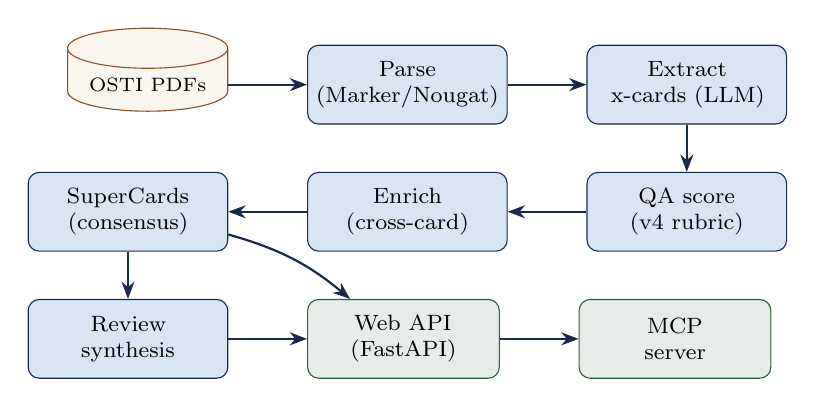
\begin{tikzpicture}[
  node distance=6mm and 10mm,
  stage/.style={rectangle, rounded corners, draw=KuklaInk, fill=KuklaSky,
    text width=2.3cm, align=center, minimum height=1.0cm, font=\footnotesize},
  store/.style={cylinder, shape border rotate=90, draw=KuklaAccent, fill=KuklaMath,
    aspect=0.25, text width=1.8cm, align=center, minimum height=1.0cm, font=\scriptsize},
  serve/.style={rectangle, rounded corners, draw=KuklaGreen, fill=KuklaGreen!12,
    text width=2.2cm, align=center, minimum height=1.0cm, font=\footnotesize},
  arr/.style={-{Stealth[length=2.2mm]}, KuklaInk, thick},
]
\node[store] (pdf) {OSTI PDFs};
\node[stage, right=of pdf] (parse) {Parse\\(Marker/Nougat)};
\node[stage, right=of parse] (extract) {Extract\\x-cards (LLM)};
\node[stage, below=of extract] (qa) {QA score\\(v4 rubric)};
\node[stage, left=of qa] (enrich) {Enrich\\(cross-card)};
\node[stage, left=of enrich] (super) {SuperCards\\(consensus)};
\node[stage, below=of super] (review) {Review\\synthesis};
\node[serve, right=of review] (web) {Web API\\(FastAPI)};
\node[serve, right=of web] (mcp) {MCP\\server};

\draw[arr] (pdf) -- (parse);
\draw[arr] (parse) -- (extract);
\draw[arr] (extract) -- (qa);
\draw[arr] (qa) -- (enrich);
\draw[arr] (enrich) -- (super);
\draw[arr] (super) -- (review);
\draw[arr] (review) -- (web);
\draw[arr] (web) -- (mcp);
\draw[arr] (super) to[bend left=12] (web);
\end{tikzpicture}
\end{center}

The canonical flow is: \textbf{OSTI corpus (PDFs)} $\rightarrow$ Marker/Nougat
parsing to \code{.md}/\code{.mmd} $\rightarrow$ LLM extraction to seven-modality
cards $\rightarrow$ QA scoring $\rightarrow$ cross-card enrichment $\rightarrow$
SuperCard merging $\rightarrow$ review-article synthesis $\rightarrow$ served through
the web API and MCP server.

\subsection{Component inventory}

The repository is organized by pipeline stage, with code only --- no data --- in the
tree. The databases and corpus live on dedicated storage (Section~\ref{sec:storage}).

\begin{center}
\small
\begin{tabular}{@{}l p{9.4cm}@{}}
\toprule
\textbf{Directory} & \textbf{Responsibility} \\
\midrule
\code{scripts/}              & Catalog build + corpus fetch (Stages 0--1) \\
\code{pipeline/extraction/}  & Parsed text $\rightarrow$ raw x-cards; sync to SQLite + FTS5 \\
\code{pipeline/quality/}     & QA scoring, URL validation, code/data-repo filters \\
\code{pipeline/enrichment/}  & Cross-card fact transfer, email mining, entity resolution \\
\code{pipeline/supercards/}  & Merge same-resource cards into consensus records \\
\code{pipeline/reviews/}     & Synthesize review/tutorial articles \\
\code{pipeline/citations/}   & OpenAlex / Semantic Scholar citation enrichment \\
\code{web/}                  & FastAPI browsing/search site + static frontend \\
\code{mcp/}                  & MCP server exposing cards to agents \\
\code{prompts/}              & All LLM prompts (extraction, enrichment, review) \\
\code{docs/}                 & Architecture, QA rubric, strategy docs, runbooks \\
\code{datasets/}             & Manifests + pointers to rebuild every data artifact \\
\code{tests/}                & End-to-end + performance tests \\
\bottomrule
\end{tabular}
\end{center}

\subsection{Why SQLite everywhere}

Every stage reads and writes SQLite. This is a deliberate choice: SQLite files are
single-file, trivially replicated (rsync/scp between hosts), support FTS5 full-text
indexing natively, and tolerate the ``one long-lived writer, many readers'' access
pattern that the pipeline exhibits. The pipeline stages are coordinated not by a
message queue but by \emph{atomic work-claiming SQL} (e.g.\ ``select rows where
\code{review\_md IS NULL}'') --- which is what makes the whole system restartable
with no external scheduler state.

\clearpage
% ======================================================================
\section{The Data Model}
% ======================================================================

Three SQLite databases carry the system's state: the \textbf{card} store, the
\textbf{SuperCard} store, and the \textbf{entity} store. A fourth (the \emph{catalog})
holds OSTI metadata and parse paths and seeds the whole pipeline.

\subsection{\code{cards} (osti\_cards.sqlite)}

One row per extracted resource-card. Key columns:

\begin{itemize}[noitemsep,topsep=2pt]
\item \code{osti\_id}, \code{year}, \code{mode}
  (data / model / agent / instrument / facility / simulation / workflow)
\item \code{title}, \code{description}, \code{yaml} (the full structured card body)
\item \code{urls}, \code{emails}, \code{authors} (JSON arrays; zero-hallucination)
\item \code{qa\_version}, \code{qa\_tier} (HIGH/MEDIUM/LOW), and the component scores
  \code{qa\_completeness}, \code{qa\_provenance}, \code{qa\_grounding},
  \code{qa\_entity\_count}, \code{qa\_missing\_fields}
\item \code{doe\_codes}, \code{doe\_subject\_names}, \code{doe\_domains}
  (official DOE OSTI subject classification)
\item \code{review\_md}, \code{review\_model}, \code{review\_at}
  (the synthesized review/tutorial article and its provenance)
\end{itemize}

An FTS5 virtual table indexes title/description/body for prefix search, and is what
both the website search box and the MCP \code{osti\_search} tool query.

\subsection{\code{supercard} (supercards.sqlite)}

One row per real-world resource, merging many cards. Kept in a \emph{sibling} DB so
the per-paper card corpus stays pristine and SuperCards can be rebuilt
independently.

\begin{itemize}[noitemsep,topsep=2pt]
\item \code{super\_id} ($=$ \code{super-<mode>-<slug>}, stable/idempotent),
  \code{canonical\_name}, \code{mode}, \code{member\_count},
  \code{first\_year}/\code{last\_year}
\item \code{consensus\_json} --- evidence-weighted field consensus with
  support/dissent counts
\item \code{urls}, \code{emails}, \code{labs} (observed across members)
\item \code{evidence} --- pre-joined member-paper descriptions, for review synthesis
\item \code{review\_md}, \code{review\_model}, \code{review\_at}
\item join table \code{supercard\_member(super\_id, osti\_id)}
\end{itemize}

\subsection{\code{entities.sqlite}}

Entity and alias resolution (names/tools/datasets) that feeds SuperCard merging.
This is the layer that decides ``Advanced Photon Source'' $=$ ``APS'' $=$ ``APS at
Argonne'' are the same resource (Section~\ref{sec:supercards}).

\subsection{The catalog (catalog.sqlite)}

The catalog's \code{papers} table is the universe and the index: \code{osti\_id},
\code{title}, \code{product\_type}, \code{year}, \code{primary\_lab},
\code{subjects\_json}, and --- critically --- \code{md\_path} and \code{mmd\_path},
the on-disk locations of the Marker and Nougat parses. The authoritative corpus
total is \textbf{234{,}705} papers, defined as \code{product\_type} $\in$
\{Journal Article, Conference, Technical Report\} --- books, theses, and the large
Materials-Project dataset records are deliberately excluded.

\begin{notebox}{A standing hazard: the catalog path drift}
After any re-shard of the parsed \code{.md}/\code{.mmd} files on disk, the catalog's
\code{md\_path}/\code{mmd\_path} columns go stale (they point at the pre-move
location). This is the single most common drift bug in the corpus. A dedicated
repair toolkit reconciles disk-vs-catalog, rewrites paths to disk truth
idempotently (backing up the catalog first), and re-shards stray files into their
\code{<year>/} directories. Any stage that writes parse paths must batch its writes
and defer rather than fight the long-lived recovery writer that holds the WAL lock.
\end{notebox}

\clearpage
% ======================================================================
\section{Stage 0--1: Catalog and Corpus Fetching}
% ======================================================================

\subsection{Building the catalog}

\code{scripts/build\_catalog.py} bulk-pulls OSTI metadata into the catalog from the
public OSTI JSON API (\code{https://www.osti.gov/api/v1/records}), parameterized by a
set of DOE labs and a year range. It iterates \code{(lab, year)}, paginates
\code{/records} at \code{rows=500} ordered by publication date, normalizes the
organization list into a \code{primary\_lab}, and UPSERTs each record into the
\code{papers} table. \code{scripts/init\_catalog.py} creates the schema first.

\begin{lstlisting}[language=bash]
python scripts/init_catalog.py
python scripts/build_catalog.py --year-start 2000 --year-end 2026 --labs ANL,ORNL
# Catalog path resolves from --catalog | $OSTI_CATALOG | data/catalog.sqlite
# OSTI etiquette: a contact email goes in the User-Agent via $OSTI_CONTACT_EMAIL
\end{lstlisting}

\subsection{Fetching full text}

\code{scripts/fetch\_osti\_corpus.py} retrieves PDFs via the OSTI PURL endpoint
(\code{https://www.osti.gov/servlets/purl/\{osti\_id\}}) plus a discovery pass, and
writes them year-sharded as \code{<year>/<osti\_id>.pdf}.

\begin{rulebox}{Network-identity constraint}
OSTI fetches must run from a host OSTI does not blackhole. A home consumer IP is
rate-limited into silent zero-byte responses; the production fetch therefore runs
from a DOE-network host (e.g.\ a CELS DGX). The PURL endpoint is itself flaky ---
off-site redirects can silently yield a 0-byte file --- so every fetch validates the
\code{\%PDF} magic header and a minimum size floor before accepting a download. The
authoritative ``do we already have this paper?'' test is a SHA-256 of the file
bytes against the manifest, \emph{never} the basename (basenames collide across
provenance caches).
\end{rulebox}

\subsection{The corpus-recovery loop}

The gap between ``papers known to exist in OSTI'' and ``PDFs physically on disk'' is
closed by an iterative recon $\rightarrow$ fetch $\rightarrow$ diagnose $\rightarrow$
recover loop. Each missing paper is placed in a WHY-bucket (PURL 404, 403, non-PDF
landing page, publisher redirect, no DOI, \ldots) and each bucket has a priority-ordered
recovery strategy (Unpaywall, OpenAlex, Semantic Scholar, direct-publisher,
browser-context CDP fetch for bot-walled publishers, institutional-IP exit node for
licensed content). A state DB owns every \code{(osti\_id, strategy, outcome)} triple
and runs strategies in order until exhaustion. Genuinely closed-access or withdrawn
records are recorded as such, not retried forever.

\clearpage
% ======================================================================
\section{Stage 2: Parsing PDFs to Text}
% ======================================================================

An LLM cannot read a PDF's layout; it reads text. Stage 2 converts each PDF into two
complementary plain-text renderings:

\begin{itemize}[noitemsep,topsep=2pt]
\item \textbf{Marker} $\rightarrow$ \code{.md} --- a fast, layout-aware Markdown
  rendering that handles headings, lists, and most tables well.
\item \textbf{Nougat} $\rightarrow$ \code{.mmd} --- a transformer OCR model
  (Meta's Nougat) that excels at mathematical notation and dense scientific
  typesetting, producing ``mathpix markdown.''
\end{itemize}

The goal is \emph{one \code{.md} and one \code{.mmd} per paper}. Having both gives
the downstream extractor a fallback: where Marker drops a table, Nougat often keeps
it, and vice-versa. Parse paths are recorded in the catalog's \code{md\_path} and
\code{mmd\_path} columns.

\subsection{Why this runs on HPC}

Parsing is the only GPU-bound stage. Marker and Nougat run on A100 (ALCF Polaris,
CELS DGX, or a local 8$\times$A100 host) and Intel PVC (Aurora) in restartable batch
jobs. The jobs follow the restartability discipline (Section~\ref{sec:engineering}):
atomic per-item work-queue claims, an external cron-driven reaper that recovers
orphaned ``running'' rows, and self-chaining resubmission to keep $N$ jobs in flight
until the pending count reaches zero. A walltime kill therefore loses only the
handful of papers in flight at that instant.

\begin{notebox}{GPU co-tenancy and the OOM cascade}
On a shared multi-GPU host, resident inference servers frequently occupy 27--55\,GB
on random GPUs. A parse worker that lands on a memory-tight GPU will OOM, and once
its CUDA context is destroyed it can mark every remaining claimed item FAILED ---
leaving orphan locks that make surviving workers exit early. The pre-flight check
queries per-GPU free memory and pins one worker per GPU with ${>}60$\,GB free via
\code{CUDA\_VISIBLE\_DEVICES}. A 0-byte \code{.mmd} from the small Nougat model is a
genuine parse bailout (repetition collapse or an image-only PDF), not a pipeline
bug; those papers are flagged for a base-model redo rather than retried in place.
\end{notebox}

\subsection{The mmd-to-PDF auto-render workflow}

For the website's ``view the source paper'' feature, parsed \code{.mmd} files are
rendered back to PDF. An operator on the serving host triggers idempotent remote
rendering over the mesh, then incrementally pulls the rendered PDFs into the site's
tree. This keeps the render farm's output flowing to the browse layer without a
monolithic batch step.

\clearpage
% ======================================================================
\section{Stage 3: x-Card Extraction}
% ======================================================================

This is the heart of the system: reading parsed text and emitting structured cards.

\subsection{The extractor and the sync}

The production extractor (the ``extract-o-matic'' family) reads a paper's parsed
text and, for each of the seven modalities present, emits a structured card.
\code{pipeline/extraction/sync\_cards.py} then syncs the farm-produced cards back to
\code{m1} and (re)builds the SQLite FTS5 index. It is idempotent --- safe to run on a
timer while extraction is still producing cards --- and it skips \code{NO\_X\_FOUND}
sentinels so that only real cards land in the DB.

\begin{rulebox}{A sharp operational edge}
\code{sync\_cards.py} \textbf{DROPS and RECREATES} the \code{cards} table on a full
sync. Enrichment, QA, and review columns are therefore applied \emph{after} a full
sync completes --- otherwise they are silently lost. The system's answer to this is
the sibling-DB pattern (SuperCards, enrichment staging, citations all live in their
own files) plus a strict stage ordering in the replication runbook.
\end{rulebox}

\subsection{Multi-entity capture}

A paper that describes three instruments must yield \emph{three} instrument entries,
not just the first. The extraction prompt emits a \emph{list} of entities per
modality, superseding the legacy single-block, first-match-only behavior. Each
entity is independently completeness-scored, and the card records its
\code{entity\_count}. Within a card, the same named entity mentioned repeatedly is
merged to one entity.

\subsection{The derived-content bracketing convention}

A global rule distinguishes paper-grounded fact from model inference:

\begin{itemize}[noitemsep,topsep=2pt]
\item \textbf{Direct} content (copied/closely paraphrased from the paper) is written
  plain.
\item \textbf{Derived} content (inferred, normalized, or synthesized) is wrapped in
  brackets with its source, e.g.\\
  \code{license: "[derived: CC-BY-4.0 from journal default]"}.
\item \textbf{Unknown} values are written \code{"UNKNOWN"} --- never guessed
  unbracketed.
\end{itemize}

A reader, and the quality scorer, can thus always tell what the paper said from what
the model inferred.

\subsection{The universal provenance block}

Every card carries a provenance block tying it back to the source:

\begin{lstlisting}[language=yaml]
source:
  osti_id: "<id>"                      # REQUIRED, direct
  title: "<paper title>"               # REQUIRED, direct
  doi: "<doi or UNKNOWN>"
  url: "<landing/pdf url or UNKNOWN>"
  authors: ["Last, First", ...]        # REQUIRED, direct
  author_emails: ["a@lab.gov", ...]    # direct if present
  affiliations: ["Argonne National Laboratory", ...]
  primary_lab: "<DOE lab or UNKNOWN>"  # derived(bracket) allowed
  funding:
    - agency: "DOE Office of Science"
      award: "DE-AC02-06CH11357"
  funding_text: "<verbatim acknowledgement>"
\end{lstlisting}

\subsection{LLM infrastructure}

Extraction and review synthesis run on the \textbf{pecans qwen3.8-27b farm} --- an
endpoint pool of roughly 17 live OpenAI-compatible \code{/v1/chat/completions}
servers, authenticated with a bearer key. Jobs are sharded with \code{--shard M/N}
(by \code{rowid \% N}) across workers and claim work atomically, so scaling is a
matter of launching more shards. A high-quality fallback path routes to Argo Sonnet
through a LiteLLM aggregator on \code{localhost:4000}. For review synthesis,
\code{enable\_thinking=False} --- the tokens should become article text, not
reasoning trace.

\clearpage
% ======================================================================
\section{Stage 4: Quality Assurance}
% ======================================================================

Every card is scored so consumers can distinguish a complete, well-grounded card
from a thin one. The scorer (\code{pipeline/quality/qa\_score.py}) computes the
deterministic/structural sub-scores; the LLM-judged grounding sub-score is computed
separately (regex is never used for judgment).

\subsection{The three sub-scores}

\begin{itemize}[noitemsep,topsep=3pt]
\item \textbf{completeness} $=$ filled required fields / total required fields,
  averaged across entities. A field is ``filled'' if non-empty and not a bare
  \code{UNKNOWN} (bracketed-derived counts as filled).
\item \textbf{provenance} $=$ weighted presence of the provenance block
  (osti\_id~.1, title~.1, authors~.2, emails~.15, affiliations~.15, funding~.3).
\item \textbf{grounding} $=$ fraction of entity-defining claims traceable to the
  parsed full text --- LLM-judged, not regex.
\end{itemize}

\subsection{The v4 HIGH gate (current definition)}

The quality definition evolved through several of Rick's corrections; the current
authoritative gate is a four-component test:

\begin{rulebox}{HIGH $=$ validated URL $+$ names $+$ email $+$ key technical info}
A card is \textbf{HIGH} when it has a validated/actionable \textbf{URL}, author
\textbf{names}, at least one author \textbf{email}, and key \textbf{technical
information}. Funding acknowledgement is explicitly \emph{not} a quality trigger
(``nice to have''). MEDIUM and LOW fall out below the respective thresholds, and any
hallucinated or ungrounded entity forces LOW. The tier is written honestly --- a LOW
card is labeled LOW; the distinction is surfaced, not hidden.
\end{rulebox}

\noindent The per-modality required-field tables (what counts toward completeness
for a \code{data} card vs.\ an \code{instrument} card vs.\ a \code{simulation} card)
are specified in \code{docs/QA\_RUBRIC.md}. For example, a \code{data} card requires
dataset name/type, short and full description, provider, license, access,
repository URL, size/format, and version; a \code{simulation} card requires code
name/type, role in paper, descriptions, developer, version, license, code URL, and
physics/inputs.

\subsection{URL validation}

\code{pipeline/quality/url\_validate.py} classifies and HTTP-verifies the URLs on
each card, setting a \code{url\_validated} flag that feeds the HIGH gate. Companion
filters (\code{code\_repo\_filter.py}, \code{data\_repo\_filter.py}) identify cards
that carry an actionable code or data repository, powering the website's
``Has code repository'' / ``Has data repository'' facets.

\subsection{The QA pipeline is non-destructive}

QA writes \emph{new} \code{qa\_*} columns and new re-extracted card versions; it
never overwrites the existing corpus. Every stage is idempotent and restartable,
claims work atomically, and writes a ledger.

\clearpage
% ======================================================================
\section{Stage 5: Enrichment}
% ======================================================================

Extraction leaves gaps: an author's email the extractor missed, a license present in
a sibling paper but not this one, a tool's developer stated in one card and absent in
another. Enrichment fills those gaps \emph{without inventing anything}.

\subsection{The measured gap}

Against a live snapshot of 232{,}035 cards / 103{,}017 papers:

\begin{center}
\small
\begin{tabular}{@{}l r l@{}}
\toprule
\textbf{Component} & \textbf{Coverage} & \textbf{Status} \\
\midrule
Names (authors)                 & 95.3\% & nearly solved \\
Actionable URL (pre-validation) & 71.0\% & validate + recover \\
Emails                          & 52.1\% of papers & 49{,}358 papers lack any email \\
Key technical info (comp.\ $\geq 0.85$) & 20.9\% & dominant limiter \\
\bottomrule
\end{tabular}
\end{center}

\noindent The most-missing technical fields corpus-wide are location (116k),
license (110k), version (69k), access (53k), and workflow steps (40k).

\subsection{The source ladder (cheapest, most trustworthy first)}

\textbf{Email sources.}
\begin{enumerate}[noitemsep,topsep=2pt]
\item \textbf{S-E1 Parse-mining} --- 61\% of email-less papers have an author email
  printed in their \emph{own} parse that the extractor missed. An author-email
  classifier mines the header/affiliation region and rejects boilerplate
  (\code{reports@*.osti.gov}, \code{webmaster@}, generic ordering addresses).
  Biggest win, zero cost, zero hallucination.
\item \textbf{S-E3 Cross-card transfer} --- the same author appearing in another
  paper that \emph{does} have their email; the observed address is transferred,
  person-name keyed.
\item \textbf{S-E4 Web} (OpenAlex / Crossref / ORCID) --- resolve the corresponding
  author to a verified email from an authoritative record; cite the source URL.
  Last resort.
\item \textbf{Never} pattern-construct \code{first.last@lab.gov}. Verified-or-empty.
\end{enumerate}

\textbf{Technical-info sources.} Re-parse-mining of fields that are in the parse but
were dropped; cross-card consensus transfer (14{,}115 named entities appear in more
than one card, covering 48\% of the corpus); cited web enrichment with live-validated
URLs; and tightly-guarded parametric facts about well-known entities (``LAMMPS is
C++'', ``APS is at Argonne'') --- never for URLs, emails, versions, or access.

\subsection{Staging, not mutation}

\code{enrich\_crosscard.py} transfers a consensus field value to member cards that
lack it, writing to a \emph{staging} table \code{card\_enrichment(osti\_id, mode,
field, value, source, support, created\_at)} --- it never mutates the \code{cards}
table. A value is transferred only when consensus support meets a minimum and the
target genuinely lacks the field; the operation is idempotent. \code{email\_mine.py}
emits JSONL of mined author emails, classifier-scored, for merge. Every enriched
value carries a bracketed provenance tag (\code{[enriched:cross-card]},
\code{[enriched:web <url>]}) so the original paper content stays visibly untouched.

\begin{notebox}{The regex hard rule}
Enrichment and QA obey a standing rule: \emph{no regex when an LLM will do better}.
Regex is permitted only for genuinely mechanical fixed-schema parsing (splitting
YAML keys, extracting a URL host). Any field that feeds a downstream judgment,
ranking, or selection --- grounding, entity detection, field derivation, email
classification --- uses the LLM. The cascade pattern keeps cost down: a cheap model
triages binary flags, a strong model does deep extraction only on the hits.
\end{notebox}

\clearpage
% ======================================================================
\section{Stage 6: SuperCards}
\label{sec:supercards}
% ======================================================================

A resource like VASP, LAMMPS, or the Advanced Photon Source is described hundreds to
thousands of times across the corpus. Each mention is partial. A \textbf{SuperCard}
is the consolidated, canonical record of \emph{one} real-world resource, synthesized
from \emph{every} card that mentions it.

\subsection{Feasibility (live corpus)}

Of 140{,}364 distinct named entities, \textbf{14{,}115 appear in more than one card}
--- these are SuperCard-eligible and cover 111{,}222 cards (48\% of the corpus). The
heavy hitters are exactly the high-value shared infrastructure: facilities (APS,
ALS, NERSC, SNS, OLCF) and codes (VASP, LAMMPS). The long tail of single-mention
entities becomes \emph{singleton} SuperCards --- still useful as the canonical entry,
but without cross-card consensus.

\subsection{The hard problem: entity resolution}

Name-exact matching is the floor but insufficient; aliases, acronyms, and versions
must be reconciled (``Advanced Photon Source'' $=$ ``APS''; ``VASP'' $=$ ``Vienna Ab
initio Simulation Package'' $=$ ``vasp 5.4''). The resolution pipeline is
\emph{blocking $\rightarrow$ matching $\rightarrow$ clustering}:

\begin{enumerate}[noitemsep,topsep=2pt]
\item \textbf{Normalize} the name (lowercase, strip version/punctuation) into a cheap
  blocking key.
\item \textbf{Alias table} --- curated plus auto-detected acronym$\leftrightarrow$
  expansion (from cards that contain both forms, e.g.\ ``Advanced Photon Source
  (APS)'').
\item \textbf{LLM adjudication within a block} (not regex) --- for candidate clusters
  sharing a key or alias, an LLM confirms ``same resource? yes/no/variant'' from the
  cards' type, developer, and description. This is the judgment step; it runs on the
  farm.
\item \textbf{Version handling} --- same base resource, different version $\rightarrow$
  one SuperCard with a \code{versions:} list (VASP 5.4 and 6.3 are one VASP
  SuperCard).
\item \textbf{Cluster $\rightarrow$ SuperCard id} $=$ \code{super-<mode>-<slug>},
  stable and idempotent.
\end{enumerate}

\subsection{Consensus synthesis}

For each cluster the canonical record is built by \emph{evidence-weighted consensus},
not concatenation. Scalar fields (developer, license, language, location) take the
value with the most support across members, recording agreement count and dissenting
values. URLs and emails are the validated union, with a canonical one promoted.
Descriptions are LLM-synthesized from the richest members. The provenance block
becomes the \emph{usage graph}: member cards, member count, first/last seen, labs,
and authors. Conflicts are surfaced (\code{license\_candidates: [...]}), never
silently averaged away. A SuperCard asserts only facts present in at least one member
card or verified via live web --- the same anti-hallucination law as enrichment.

\subsection{SuperCards as a first-class website category}

SuperCards are a separate, first-class browse category on the site, distinct from
per-paper cards, with their own search, filter, and detail pages. A SuperCard detail
page shows the consensus record plus the list of member papers (the usage graph), and
the MCP server exposes \code{supercard\_search}/\code{supercard\_get}. SuperCards also
feed the knowledge graph as canonical nodes with member cards as edges.

\clearpage
% ======================================================================
\section{Stage 7: Review/Tutorial Article Synthesis}
% ======================================================================

A card's structured fields are for machines. For humans (and for grounding an agent's
reasoning), each card and SuperCard also renders as a \textbf{review/tutorial
article} --- flowing explanatory prose, not a sparse outline of fields.

\subsection{The synthesizer}

\code{pipeline/reviews/review\_synth.py} runs on the qwen3.8-27b farm. It supports two
kinds:

\begin{lstlisting}[language=bash]
# SuperCards first (best evidence):
python pipeline/reviews/review_synth.py --kind super --workers 34
# then individual cards, sharded across workers:
python pipeline/reviews/review_synth.py --kind card --shard 0/4 --workers 20   # x4
\end{lstlisting}

It is restartable (atomic claim via \code{review\_md IS NULL}), zero-hallucination,
and runs with \code{enable\_thinking=False}. SuperCard articles are synthesized first
because they have the richest evidence; individual-card articles follow, sharded by
\code{rowid \% N}.

\subsection{Per-modality section templates}

The article structure differs by modality --- a dataset review is not a facility
review. The templates are defined in code and mirrored in \code{prompts/}. For
example:

\begin{center}
\small
\begin{tabular}{@{}l p{9.2cm}@{}}
\toprule
\textbf{Modality} & \textbf{Section template} \\
\midrule
\code{data} & Overview · What the Dataset Contains · How It Is Used in Research ·
  Access \& Format · How to Work With It (tutorial) · Provenance \& Citation \\
\code{simulation} & Overview · Method \& Physics · How It Is Used in This Corpus ·
  Capabilities \& Numerics · Typical Workflow (tutorial) · Access \& Licensing \\
\code{facility} & Overview · Capabilities \& Instruments · Science Enabled ·
  How Researchers Use It · How to Get Access (tutorial) · Operation \& Stewardship \\
\code{model} & Overview · Architecture \& Method · What It Predicts/Does ·
  How It Is Used · How to Use It (tutorial) · Access \& Licensing · Representative Works \\
\bottomrule
\end{tabular}
\end{center}

\subsection{The prompt contract}

The individual-card prompt builder (verbatim from the pipeline) feeds the paper
description and the extracted YAML as source facts, instructs the model not to
contradict them but to expand into prose, and enforces the rules:

\begin{lstlisting}[language=bash]
Write a substantive review/tutorial article in Markdown with these sections:
{per-modality sections}

Rules:
- Flowing explanatory PROSE like a tutorial - NOT a bullet outline, NOT sparse.
- Explain what the resource is, how it works, how a researcher would use it.
- Do NOT invent URLs, versions, emails, or facts absent from the description/card.
- 350-600 words (cards) / 600-900 words (SuperCards). Start with: "# {title}".
\end{lstlisting}

Articles carry inline \code{[OSTI:id]} citations so every synthesized claim points
back to the paper(s) it came from, and the website renders those as citation chips
that link to the source card.

\clearpage
% ======================================================================
\section{Stage 8: Citation Enrichment}
% ======================================================================

To let users rank and weight resources by scholarly impact, each paper's citation
count is fetched from OpenAlex (with Semantic Scholar as a secondary source), keyed
on DOI, into \code{citations.sqlite}.

\begin{rulebox}{Citation counts are fetched, never guessed}
Citation counts come exclusively from OpenAlex / Semantic Scholar keyed on the DOI
--- an LLM is \emph{never} asked how many times a paper was cited. OpenAlex enforces a
per-IP daily budget; when the serving host is capped the fetch runs from a
fresh-quota institutional IP. Likewise, science-domain classification comes from the
authoritative DOE OSTI subject codes (\code{subjects\_json} in the catalog), mapped
to domains such as Biology, HEP, Materials, Fusion, and Computer Science --- not from
LLM free-text classification.
\end{rulebox}

% ======================================================================
\section{Stage 9: The Serving Layer}
% ======================================================================

The read side is two components over the same SQLite stores: a human-facing web app
and a machine-facing MCP server.

\subsection{The web API (\code{web/app.py})}

A FastAPI + uvicorn service on port 8094, bound \code{0.0.0.0}, backed by the card DB's
FTS5 index and the SuperCard DB. Its route surface:

\begin{center}
\small
\begin{tabular}{@{}l p{8.6cm}@{}}
\toprule
\textbf{Route} & \textbf{Purpose} \\
\midrule
\code{/api/stats}                      & Corpus totals + breakdown by mode and year \\
\code{/api/search}                     & FTS5 search with mode/year/repo facets \\
\code{/api/card/\{year\}/\{mode\}/\{id\}} & Full card (all fields + YAML) \\
\code{/api/download/...}               & Download one card's YAML \\
\code{/api/bulk}                       & Bulk export of a filtered set (zip) \\
\code{/api/sources/\{year\}/\{id\}}    & Which source artifacts exist (PDF/.md/.mmd) \\
\code{/api/pdf, /api/raw, /api/render, /api/renderpdf} & Serve original PDF, raw parse, or rendered view \\
\code{/api/supercards/stats}           & SuperCard totals + by-mode breakdown \\
\code{/api/supercards/search}          & Search SuperCards (min-member filter) \\
\code{/api/supercard/\{super\_id\}}    & SuperCard detail + member papers \\
\code{/api/access/stats}               & Access-log analytics \\
\bottomrule
\end{tabular}
\end{center}

A middleware logs every request durably to \code{access\_log.sqlite} (recovering the
real client IP), surfaced via \code{/api/access/stats}. The static frontend
(\code{index.html}, \code{supercards.html}, \code{examples.html}) renders review
articles as the primary view, with the structured YAML available on demand.

\subsection{The MCP server (\code{mcp/mcp\_server.py})}

The MCP server wraps the \emph{same} FTS5 index and source-artifact store that powers
the website, so agent tools behave identically to the HTTP API. It uses the MCP 2.x
SDK over streamable-HTTP (or stdio for local dev) and exposes:

\begin{itemize}[noitemsep,topsep=2pt]
\item \code{osti\_stats} --- corpus-wide statistics and breakdowns
\item \code{osti\_search} --- FTS5 prefix search over title/description, with
  mode/year filters
\item \code{osti\_get\_card} --- one full card (all fields incl.\ complete YAML)
\item \code{osti\_get\_paper\_cards} --- every card for a single paper
\item \code{osti\_paper\_text} --- the parsed full text of the baseline paper
  (\code{md} or \code{mmd})
\item \code{osti\_list\_sources} --- which artifacts exist for a paper
\item \code{osti\_bulk\_export} --- base64 bulk export of a filtered set
\end{itemize}

\subsection{Deployment and access}

The web service runs under a \code{launchd} job with \code{KeepAlive}; it is recycled
with a \code{launchctl kickstart}. Public access is via a Tailscale Funnel hostname
(no VPN required for external users); the tailnet address serves internal clients.
Private network details are never committed to the public repository --- endpoint
references use the Funnel hostname only.

\clearpage
% ======================================================================
\section{Engineering Principles}
\label{sec:engineering}
% ======================================================================

Four disciplines recur at every stage and are worth stating on their own.

\subsection{Zero hallucination}

The system's credibility rests on this. Emails, URLs, and versions are recorded only
when observed in the paper text, a sibling card, or a verified contact DB. The one
previously-used contact database is now exhausted, so the live sources are
parse-mining, cross-card transfer, and cited web resolution. Pattern-constructed
addresses (\code{first.last@lab.gov}) are forbidden outright --- the policy is
verified-or-empty. Derived values are always bracketed with their source so a reader
can separate fact from inference.

\subsection{Restartability and chainability}

Every long-running stage is designed for a walltime kill: atomic per-item work
claims, an external reaper that recovers orphaned ``running'' rows, and self-chaining
resubmission that keeps $N$ jobs in flight until pending reaches zero. No stage
relies on a job epilogue for chaining (a walltime SIGKILL never runs the epilogue).
This is why the pipeline can run unattended across HPC queues with hard walltime
caps.

\subsection{Replace-on-improvement and non-destructive writes}

Enrichment never regresses a good card. QA and enrichment write \emph{new} columns
and \emph{staging} tables rather than overwriting the card corpus; superseded cards
remain, versioned. The one destructive operation (the \code{sync\_cards.py} table
rebuild) is fenced by strict stage ordering and the sibling-DB pattern so that
derived work is never collaterally destroyed.

\subsection{Honest tiering and provenance}

A LOW card is labeled LOW. Quality tiers are surfaced, not hidden, so a consumer can
choose a precision/recall point. Every fact traces to a source OSTI record, every
enriched value to its enrichment source, every review claim to the paper it came
from. Three-tier corpus replication (a primary external drive, a DGX shared-storage
mirror, and purgeable HPC scratch) protects the bytes; the derived DBs are
rebuildable from the corpus at any time.

\subsection{Storage and durability}
\label{sec:storage}

The source PDFs are stored year-sharded (\code{<year>/<osti\_id>.pdf}) with the
primary copy on a dedicated external drive, a mirror on DGX shared storage, and
scratch staging on HPC. The catalog ($\sim$1.5\,GB) and the parsed \code{.md}/\code{.mmd}
co-locate with the PDFs. The derived databases --- cards ($\sim$2.7\,GB), SuperCards
($\sim$192\,MB), entities ($\sim$144\,MB), citations, enrichment staging --- are the
pipeline's output and can be regenerated from the corpus. No data lives in the Git
repository; \code{datasets/} holds only manifests and pointers.

\clearpage
% ======================================================================
\section{Replication: Rebuilding the Stack from Zero}
% ======================================================================

The complete from-scratch sequence, each stage restartable:

\begin{center}
\small
\begin{tabular}{@{}r l l@{}}
\toprule
\textbf{Stage} & \textbf{Command} & \textbf{Produces} \\
\midrule
0 & \code{scripts/build\_catalog.py}             & catalog.sqlite \\
1 & \code{scripts/fetch\_osti\_corpus.py}        & \code{<year>/<id>.pdf} \\
2 & Marker + Nougat (GPU batch)                  & \code{.md} / \code{.mmd} \\
3 & \code{extraction/sync\_cards.py}             & osti\_cards.sqlite + FTS5 \\
4 & \code{quality/qa\_score.py}, \code{url\_validate.py} & qa\_* columns \\
5 & \code{enrichment/entity\_resolve.py}, \code{enrich\_crosscard.py}, \code{email\_mine.py} & entities + staging \\
6 & \code{supercards/supercards\_build.py}       & supercards.sqlite \\
7 & \code{reviews/review\_synth.py}              & review\_md \\
8 & \code{citations/citation\_fetch.py}          & citations.sqlite \\
9 & \code{uvicorn app:app}; \code{mcp\_server.py} & live site + MCP \\
\bottomrule
\end{tabular}
\end{center}

\noindent Prerequisites: a Python 3.13 venv (\code{pip install -r web/requirements.txt}),
access to the qwen3.8-27b farm or the Argo aggregator, a few hundred GB for the
corpus plus $\sim$3.5\,GB for derived DBs, and A100/PVC GPU access for parsing.
Verification runs \code{tests/test\_site\_e2e.py} and spot-checks
\code{/api/stats} and \code{/api/supercards/stats}.

\begin{notebox}{Critical ordering constraint}
Because \code{sync\_cards.py} drops and recreates the \code{cards} table, Stages 4--8
must run \emph{after} a full extraction sync completes --- or the enrichment, QA, and
review work will be lost. The sibling-DB layout (SuperCards, enrichment, citations in
their own files) is what makes this safe in practice.
\end{notebox}

% ======================================================================
\section{Discussion and Future Work}
% ======================================================================

OSTI-x-CARDS demonstrates that a large, heterogeneous scientific corpus can be turned
into a structured, agent-actionable resource catalogue under a strict
zero-hallucination regime, at a scale (hundreds of thousands of cards) that is only
feasible with a parallel LLM farm and a restartable, SQLite-coordinated pipeline. The
dominant remaining limiter is \emph{key technical information} completeness
($\sim$21\% of cards at the HIGH bar), which the enrichment thread attacks through
re-parse-mining and cross-card consensus transfer. Each percentage point of HIGH\%
is required to be traceable to a named enrichment module and a verifiable source ---
no point earned by relabeling or fabricated fields.

Active and planned directions include: completing the author-email parse-mining pass
(which recovers $\sim$30k papers at zero marginal cost); maturing entity resolution
from exact-name blocking through alias expansion to LLM adjudication so SuperCard
clusters are clean; auto-propagating a SuperCard's validated URL/email back to member
cards to raise their tier; and feeding the SuperCard layer into a knowledge graph
where resources are canonical nodes and papers are edges. The architecture is built
so each of these consumes the \emph{same} entity-resolution and consensus layer built
once --- enrichment and SuperCards are mutually reinforcing, not parallel efforts.

\vspace{1em}
\begin{center}
\small\color{KuklaInk}
\rule{0.4\textwidth}{0.4pt}\\[4pt]
\textbf{Repository:} \href{https://github.com/rick-stevens-ai/OSTI-x-CARDS}{github.com/rick-stevens-ai/OSTI-x-CARDS}\\
Source material: U.S.\ DOE OSTI public records (\href{https://www.osti.gov}{osti.gov}).\\
All facts traceable; nothing fabricated.
\end{center}

\end{document}
